%Einleitende Worte zum Thema "Didaktisches Prinzip".\cite{bruner}
Eine Argumentationsgrundlage dieser Arbeit ist die Definition einer \emph{fundamentalen Idee} nach Schwill \cite{schwill1}. In seiner Arbeit untersucht er die philosophische Sicht der \emph{Idee} nach Plato und Kant, und formuliert diese mit den \emph{Strukturen} nach J.S. Bruner \cite{bruner} zur fundamentalen Idee. J.S. Bruner hat das didaktische Prinzip an den Strukturen der zugrundeliegenden Wissenschaft, an denen sich der Unterricht orientieren soll, formuliert.

\begin{quote}   
{\itshape "'Eine \textbf{fundamentale Idee} (bezgl. einer Wissenschaft) ist ein Denk-, Handlungs-, Beschreibungs- oder Erkl�rungsschema, das
\begin{enumerate}
	\item in verschiedenen Bereichen (der Wissenschaft) vielf�ltig anwendbar oder erkennbar ist (Horizontalkriterium),
	\item auf jedem intellektuellen Niveau aufgezeigt und vermittelt werden kann (Vertikalkriterium),
  \item in der historischen Entwicklung (der Wissenschaft) deutlich wahrnehmbar ist und l�ngerfristig relevant bleibt (Zeitkriterium),
  \item einen Bezug zu Sprache und Denken des Alltags und der Lebenswelt besitzt (Sinnkriterium)."'
\end{enumerate}}
\end{quote}

\begin{figure}[h]
	\centering
	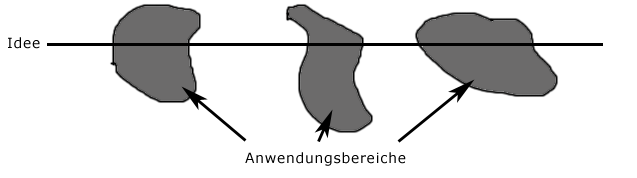
\includegraphics[scale=0.4]{graphics/horizontalkriterium.png}
	\caption{Horizontalkriterium nach \cite{schwill1}}
	\label{fig:horizontalkriterium}
\end{figure}

Das \emph{Horizontalkriterium} veranschaulicht Schwill wie in Abbildung \ref{fig:horizontalkriterium}. Eine Idee wird soweit abstrahiert, dass fachspezifische Elemente herausfallen. Damit kann themen- und fach�bergreifend gearbeitet werden. Der Lernende erkennt durch immer wiederkehrende Prinzipien die �bergreifende Relevanz der Thematik. Anschlie�end wird durch Wiederholung das Wichtige gefestigt. Die gemeinsame Idee kann jedoch wiederum nur durch umfassendes Spezialwissen herausgearbeitet werden. Das ist die Aufgabe der Lehrkr�fte.

Das \emph{Vertikalkriterium} kann wie ein Faden im Bildungsweg gesehen werden. Diesem Faden wird im Laufe der Ausbildung gefolgt. Dabei steigen das Niveau und die Detaillierung der Materie (Abbildung \ref{fig:vertikalkriterium}).

\begin{figure}[h]
	\centering
	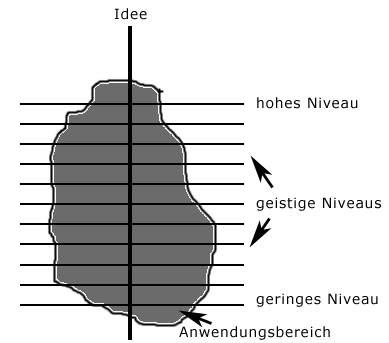
\includegraphics[scale=0.4]{graphics/vertikalkriterium.png}
	\caption{Vertikalkriterium nach \cite{schwill1}}
	\label{fig:vertikalkriterium}
\end{figure}

Das \emph{Zeitkriterium} ist in der Informatik nicht schwer zu erf�llen. Die Schnelllebigkeit der Technik birgt zwar viele Modeerscheinungen, jedoch sichert das Kriterium die Kontinuit�t des Unterrichts und den Wert der Kenntnisse und Erfahrungen der Unterrichtenden und verhindert fachliche Moden.\cite{misc:Modrow}

%\begin{quote}   
%{\itshape "'Das Kriterium sichert die Kontinuit�t des Unterrichts und den Wert der Kenntnisse und Erfahrungen der %Unterrichtenden und verhindert fachliche Moden."'}\cite{misc:Modrow}
%\end{quote}

Dabei ist die Tr�gheit der Lehre eine Art Vorauslese, um das Zeitkriterium einer fundamentalen Idee zu erf�llen.

Der Autor interpretiert das \emph{Sinnkriterium} als das tats�chliche Wertempfinden beim Empf�nger der Idee, beim Lernenden. Wie gut kann die Thematik als praxisrelevant oder als sinnvoll erkannt werden? Kann der Bezug zur sp�teren Verwendung in der Arbeitswelt hergestellt werden?

Der Einsatz fundamentaler Ideen wird von \cite{misc:Modrow} wie folgt beschrieben:

\begin{quote}   
{\itshape "'Der Unterricht muss dann so angelegt werden, dass sich diese - wenigen - fundamentalen Ideen bei den Sch�lerinnen und Sch�lern bilden k�nnen, er muss Kenntnisse und Erfahrungen vermitteln, die anhand dieser Ideen zu ordnen sind, und er muss diese Ideen zu einem geeigneten Zeitpunkt explizit thematisieren, um die spezifischen M�glichkeiten und Beschr�nkungen der Informatik in Abgrenzung gegen andere Disziplinen erkennbar zu machen."'}
\end{quote}

Einige Beispiele fundamentaler Ideen und die dazugeh�rigen Kriterien sind in \cite{schwill2} zu finden.